% =============================================================================
% Results (slides 9–13, ~6 min)
% =============================================================================

% --- Slide 9: Main result ---
\begin{frame}{Main result: +2.61 pp over SMOTE}
\begin{columns}[c]
\begin{column}{0.31\textwidth}
\begin{headline}
\bignumber{$+2.61$ pp}{macro F1 vs.\ SMOTE\\(soft-weighted)}
\end{headline}

\vspace{0.4em}
\small
\begin{itemize}\setlength\itemsep{1pt}
  \item $p < 0.0001$ \srctag{Bonferroni}
  \item Cohen's $d = 0.95$ \srctag{large}
  \item Win rate $= 88.9\%$
  \item 95\% CI $[+1.98,\ +3.25]$
\end{itemize}
\end{column}
\begin{column}{0.69\textwidth}
\centering
% Delta vs SMOTE with bootstrap 95% CIs (paper, Table I); N = 63 paired comparisons
\begin{tikzpicture}
\begin{axis}[
  lacci hbar, width=5.5cm, height=6.1cm,
  xmin=-0.8, xmax=3.4, xtick={-0.5,0,0.5,1,1.5,2,2.5,3},
  xticklabels={$-0.5$,0,,1,,2,,3},
  ymin=1, ymax=9, ytick={1,...,9},
  yticklabels={\textbf{Soft-weighted (ours)}, \textbf{Binary filter (ours)}, No augmentation,
               Embedding mixup, Back-translation, EDA, Random oversample, BERT contextual, T5 paraphrase},
  xlabel={$\Delta$ macro F1 vs.\ SMOTE (pp), with 95\% CI},
  bar shift=0pt, clip=false,
  error bars/error bar style={uaibluedark!70, line width=0.6pt},
  error bars/error mark options={rotate=90, mark size=1.8pt, uaibluedark!70, line width=0.6pt},
]
  \addplot[fill=methodOurs, draw=none, error bars/.cd, x dir=both, x explicit]
    coordinates {(2.61,1) += (0.64,0) -= (0.63,0)};
  \addplot[fill=methodOurs!60, draw=none, error bars/.cd, x dir=both, x explicit]
    coordinates {(2.39,2) += (0.68,0) -= (0.64,0)};
  \addplot[fill=methodOther, draw=none, error bars/.cd, x dir=both, x explicit]
    coordinates {(0.64,3) += (0.25,0) -= (0.22,0)
                 (-0.01,4) += (0.12,0) -= (0.12,0)
                 (-0.07,5) += (0.33,0) -= (0.35,0)
                 (-0.15,6) += (0.42,0) -= (0.42,0)
                 (-0.16,7) += (0.18,0) -= (0.19,0)
                 (-0.26,8) += (0.28,0) -= (0.32,0)
                 (-0.35,9) += (0.24,0) -= (0.27,0)};
  \vzero[methodSMOTE, dashed, thick]
  \node[font=\scriptsize\bfseries, color=methodSMOTE, anchor=south] at (axis cs:0,0.25) {SMOTE};
  % value + win-rate columns
  \colat[colhead]{0.95cm}{0.25}{$\Delta$}
  \colat[colhead]{1.9cm}{0.25}{win}
  \colat[colnum ours]{0.95cm}{1}{$+2.61$}  \colat[colnum ours]{1.9cm}{1}{88.9\%}
  \colat[colnum ours]{0.95cm}{2}{$+2.39$}  \colat[colnum ours]{1.9cm}{2}{79.4\%}
  \colat{0.95cm}{3}{$+0.64$}  \colat{1.9cm}{3}{73.0\%}
  \colat{0.95cm}{4}{$-0.01$}  \colat{1.9cm}{4}{44.4\%}
  \colat{0.95cm}{5}{$-0.07$}  \colat{1.9cm}{5}{57.1\%}
  \colat{0.95cm}{6}{$-0.15$}  \colat{1.9cm}{6}{52.4\%}
  \colat{0.95cm}{7}{$-0.16$}  \colat{1.9cm}{7}{39.7\%}
  \colat{0.95cm}{8}{$-0.26$}  \colat{1.9cm}{8}{46.0\%}
  \colat{0.95cm}{9}{$-0.35$}  \colat{1.9cm}{9}{38.1\%}
\end{axis}
\end{tikzpicture}
\end{column}
\end{columns}

\keymessage{Modern baselines (T5, BERT, mixup) do \emph{not} beat SMOTE; filtered LLM data does.}
\end{frame}

% --- Slide 10: t-SNE ---
\begin{frame}{What the filter does: emotion dataset, 10-shot}
\centering
\begin{columns}[T,onlytextwidth]
\begin{column}{0.495\textwidth}
\centering
{\small\bfseries\color{uaibluedark} Before: all LLM candidates ($\times$)}\\[2pt]
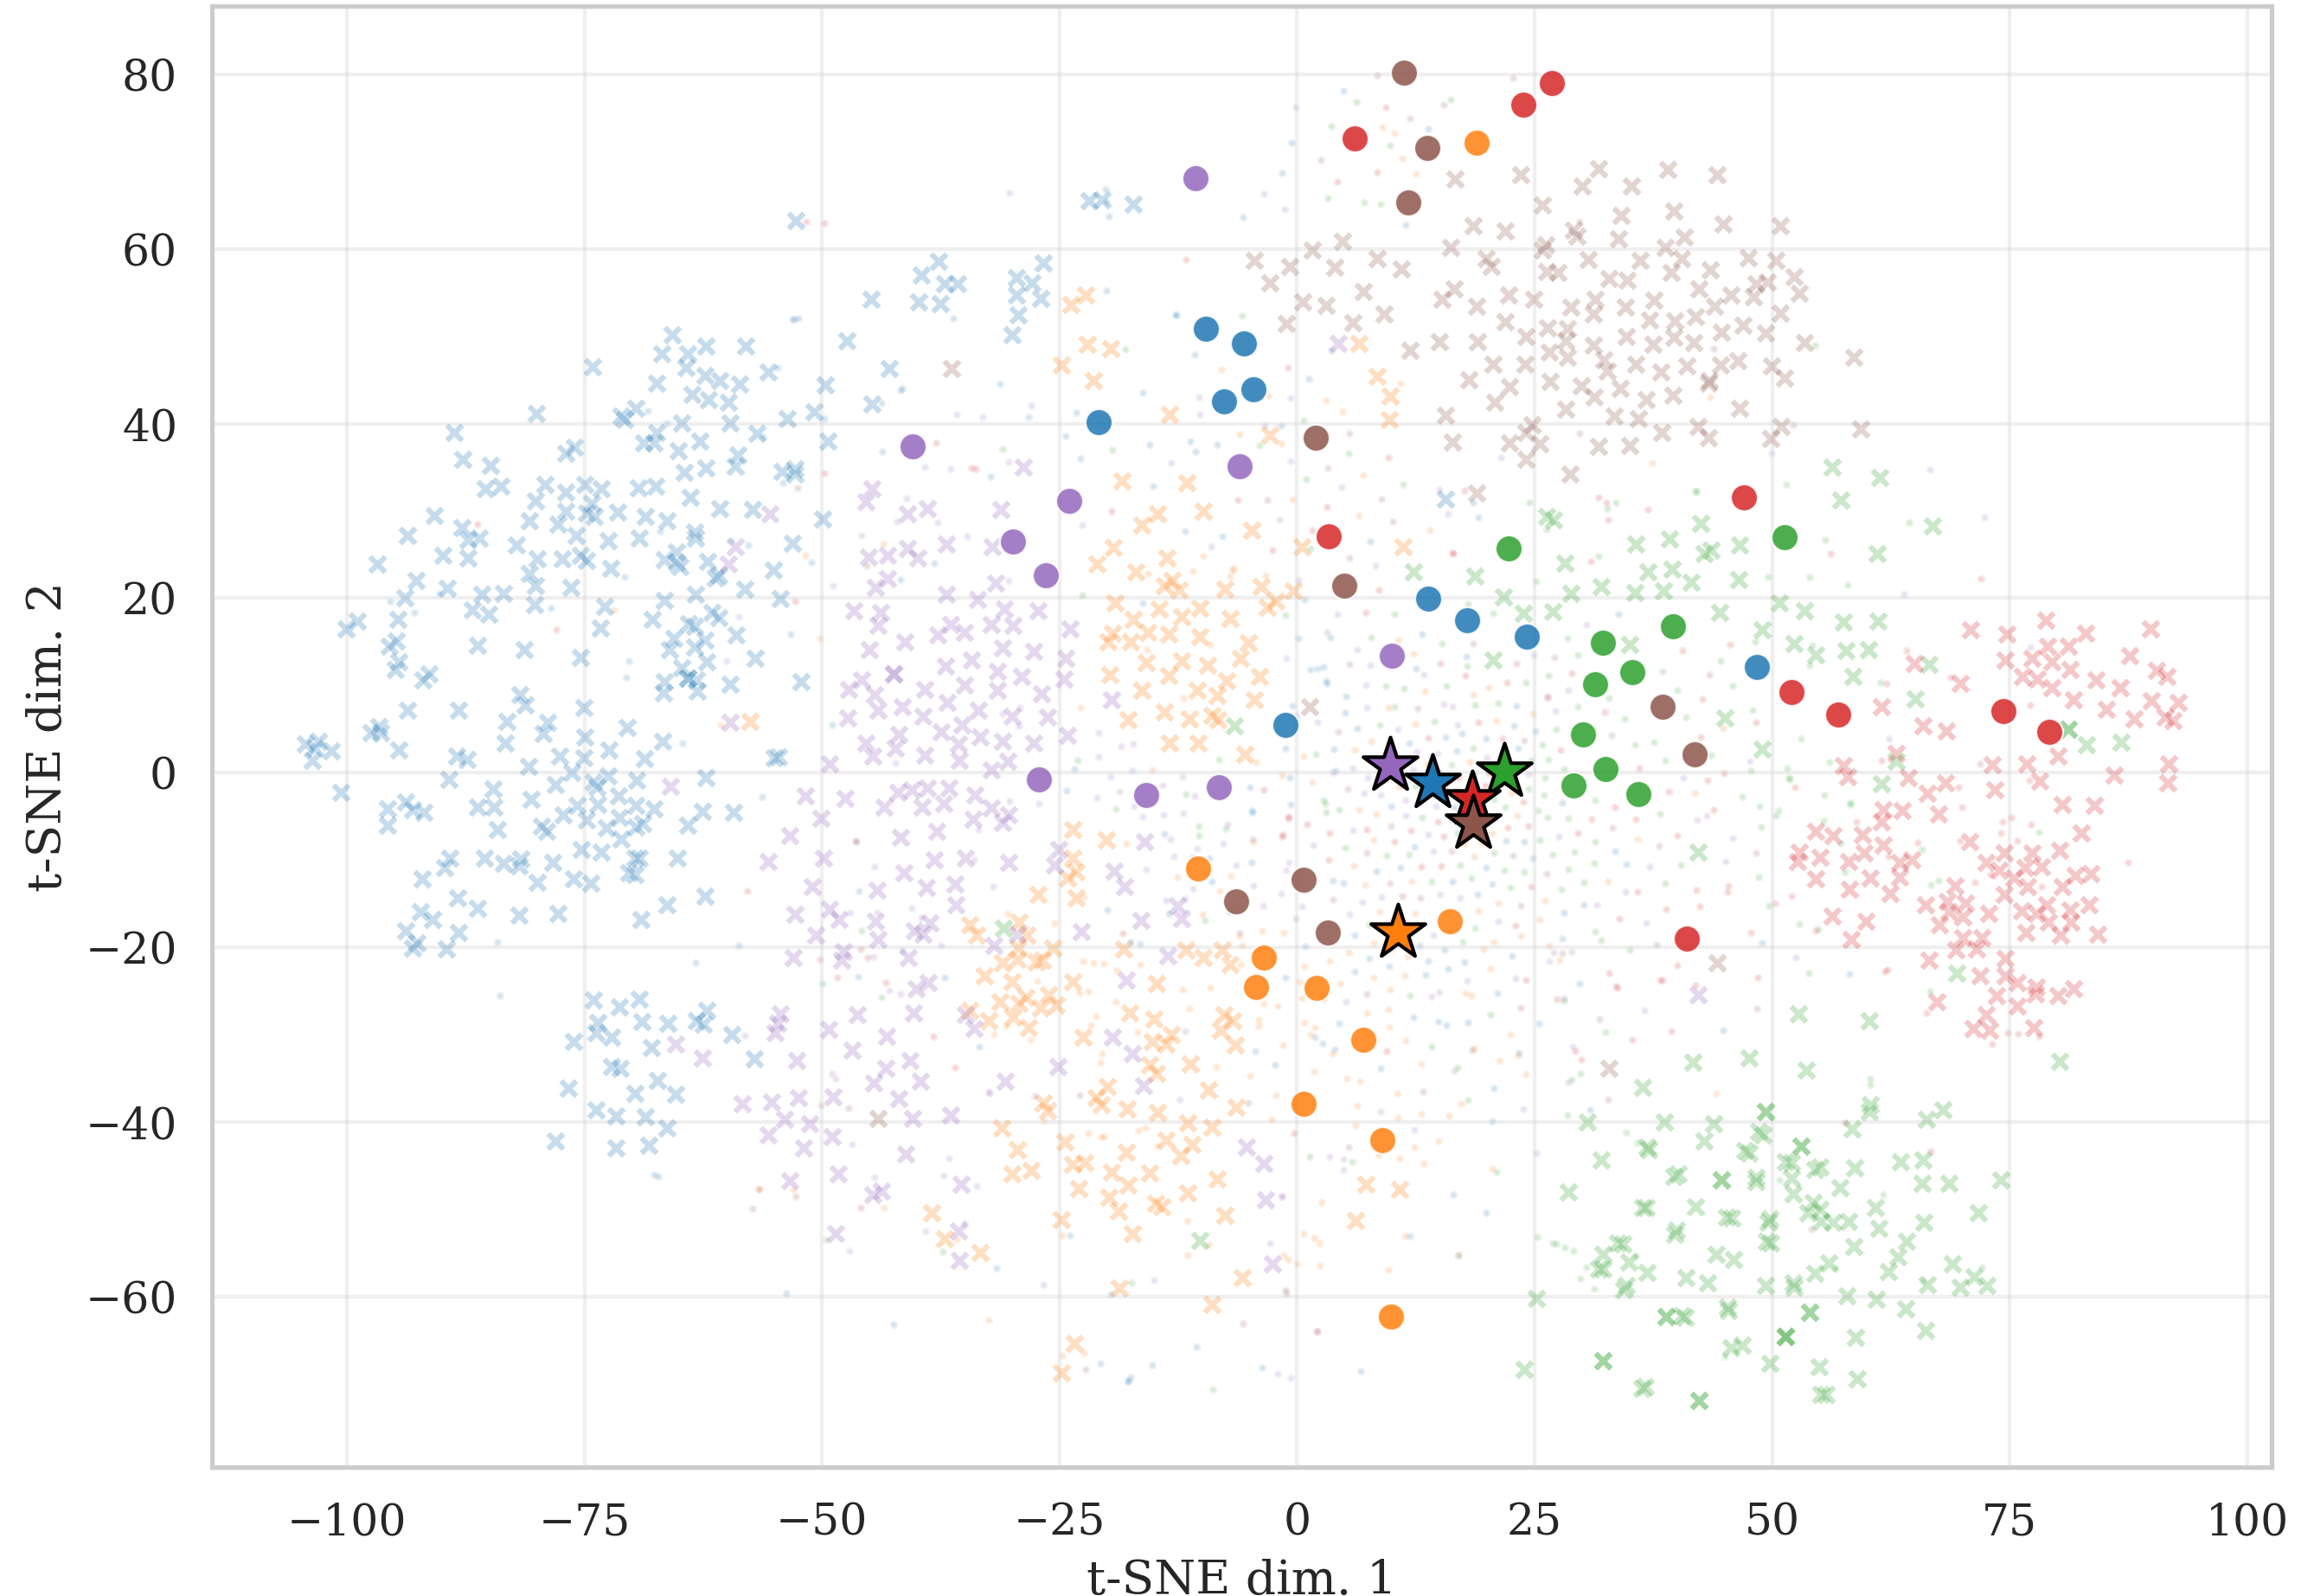
\includegraphics[width=\linewidth]{fig_tsne_emotion_before.png}
\end{column}
\begin{column}{0.495\textwidth}
\centering
{\small\bfseries\color{uaibluedark} After: kept by cascade L1 ($\blacktriangle$)}\\[2pt]
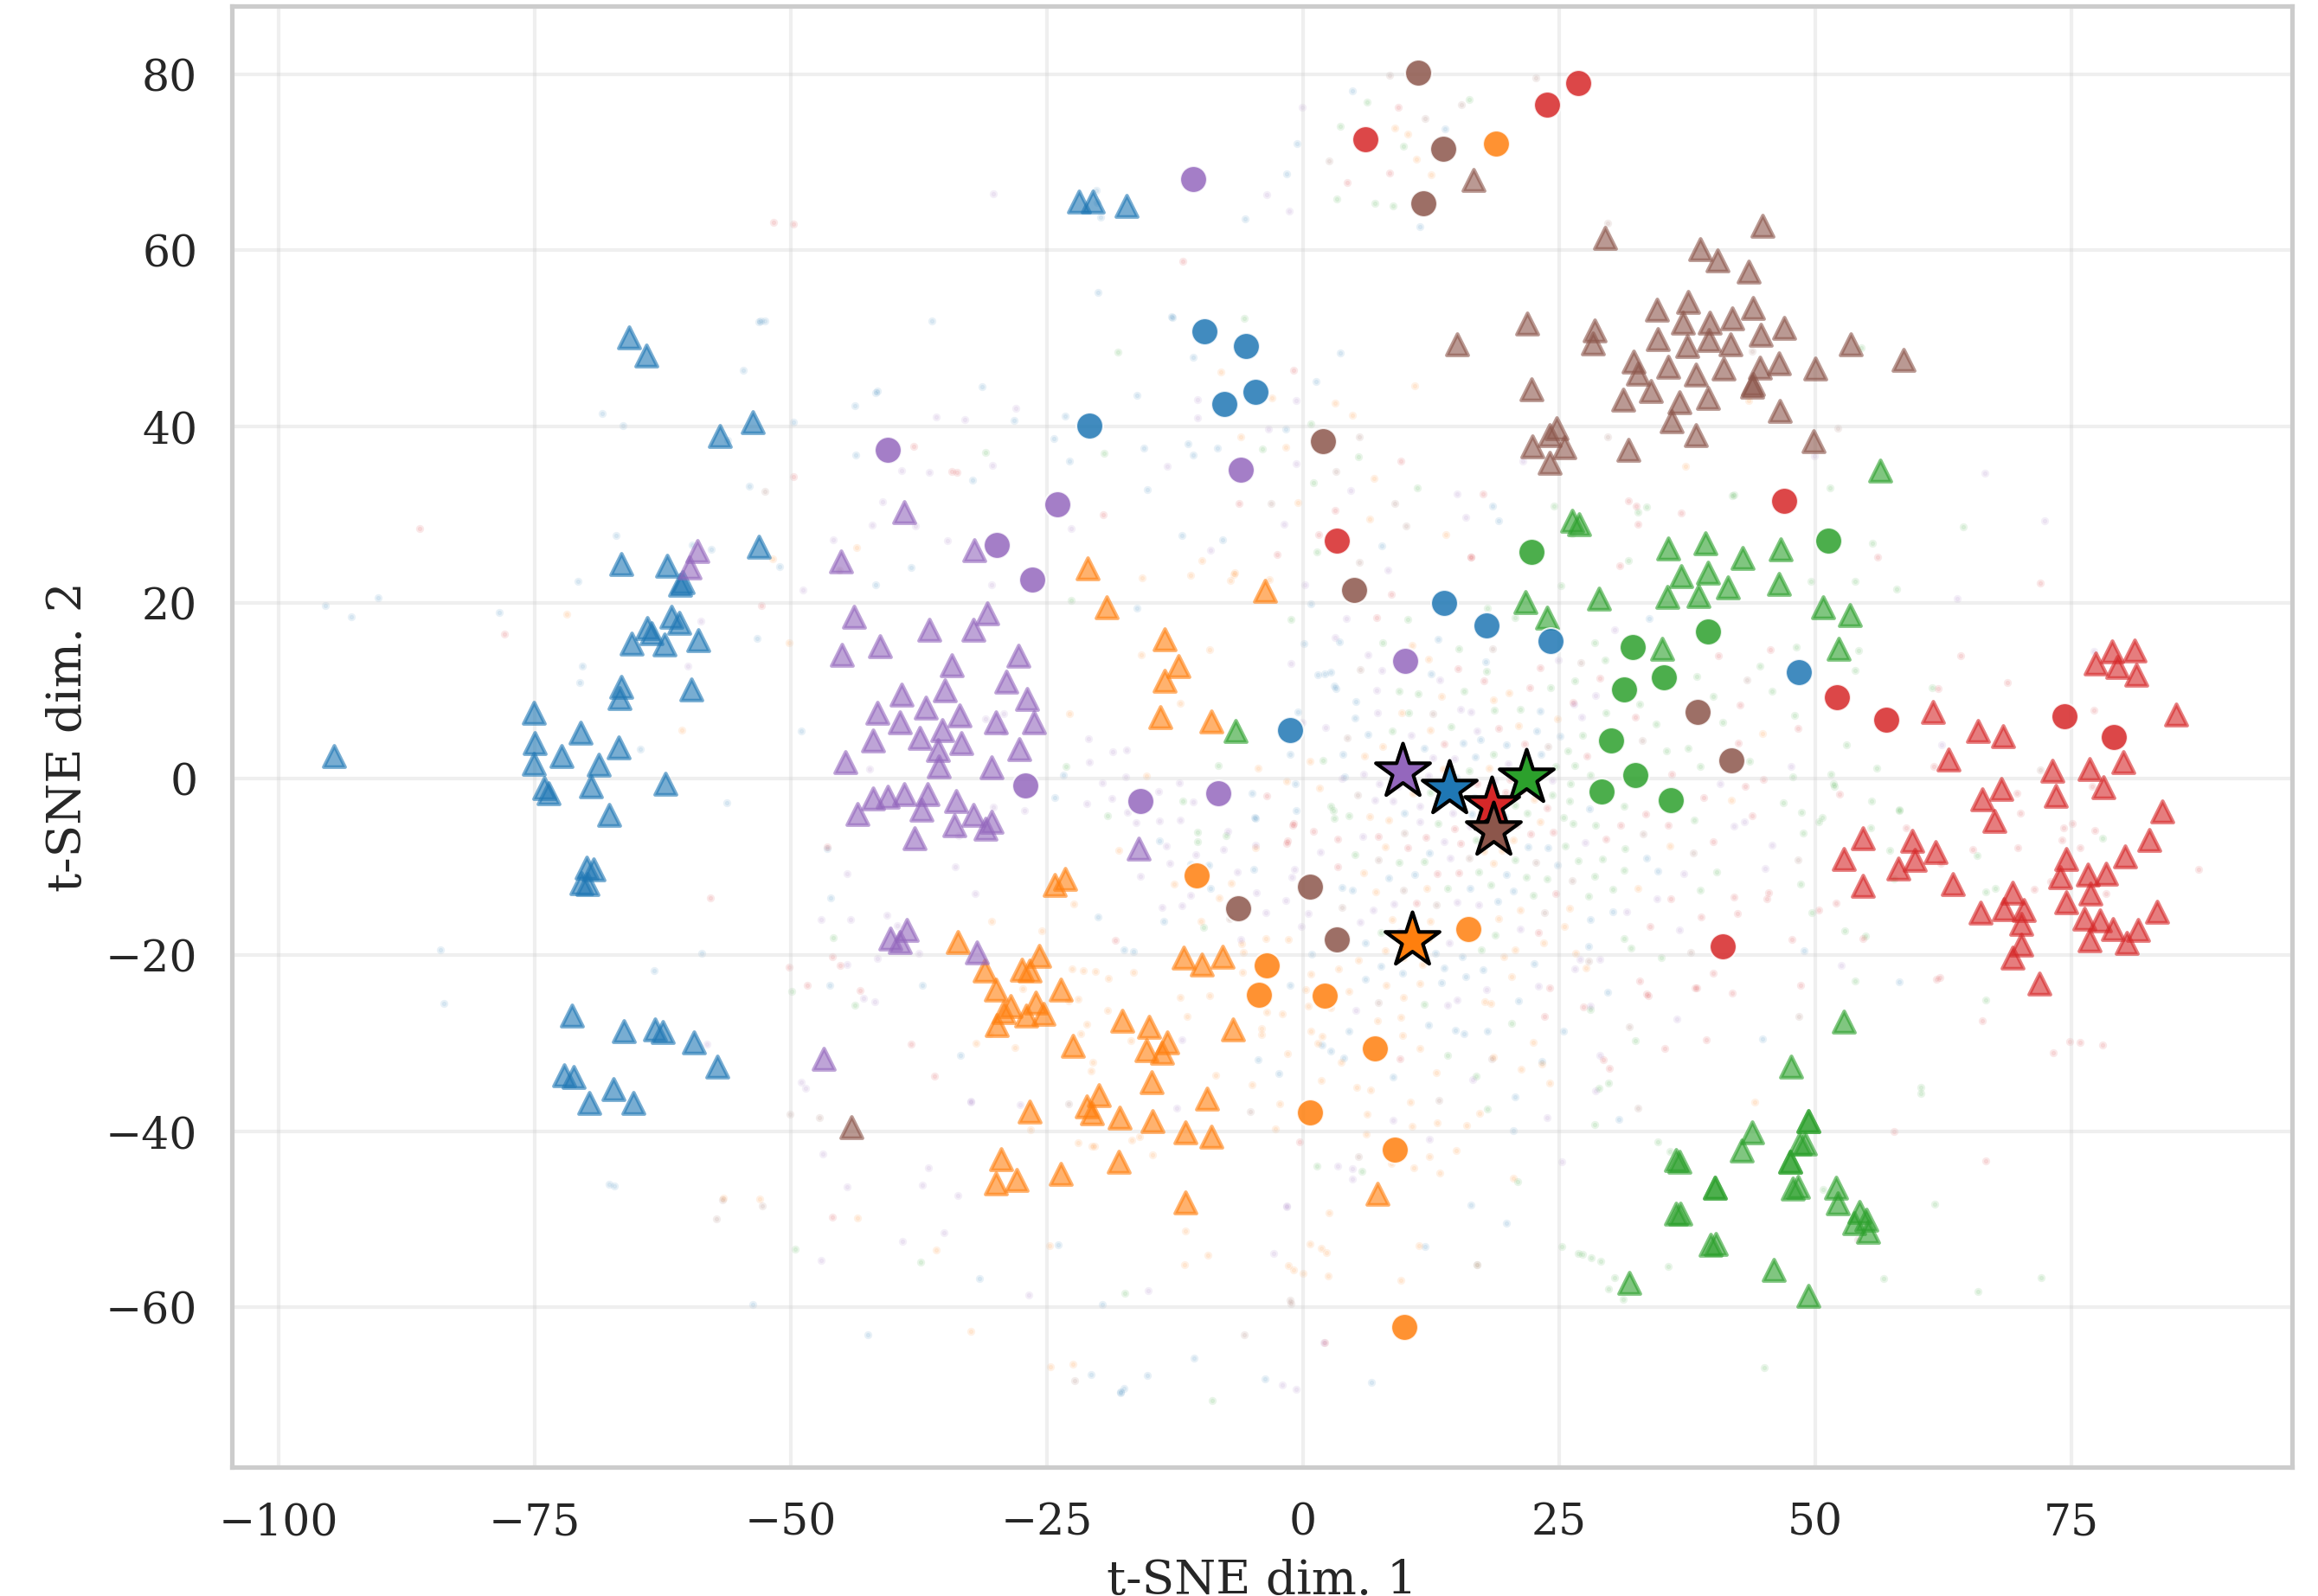
\includegraphics[width=\linewidth]{fig_tsne_emotion_after.png}
\end{column}
\end{columns}

\begin{tikzpicture}
  \foreach \c/\n [count=\i from 0] in {tabblue/anger, taborange/fear, tabgreen/joy,
                                       tabred/love, tabpurple/sadness, tabbrown/surprise} {
    \node[sw=\c] at (\i*1.3,0) {};
    \node[legendtxt] at (\i*1.3+0.1,0) {\n};
  }
  \begin{scope}[xshift=8.3cm]
    \node[legendtxt] at (0,0) {$\bullet$ real \quad $\times$ candidate \quad $\blacktriangle$ kept \quad $\bigstar$ centroid};
  \end{scope}
\end{tikzpicture}

\keymessage{Cross-class and peripheral candidates are discarded; class regions get denser.}
\end{frame}

% --- Slide 11: n-shot + classifiers ---
\begin{frame}{Largest gains where data is scarcest}
\begin{columns}[T]
\begin{column}{0.46\textwidth}
\centering
{\small\bfseries\color{uaibluedark} By examples per class}\\[2pt]
\begin{tikzpicture}
\begin{axis}[
  lacci vbar, width=6.2cm, height=5.0cm, bar width=24pt,
  ymin=0, ymax=6, ytick={0,2,4,6},
  ylabel={$\Delta$ vs.\ SMOTE (pp)},
  symbolic x coords={10,25,50}, xtick=data, enlarge x limits=0.25,
  xticklabels={{\textbf{10-shot}\\\tiny $d=1.48$\\\tiny win 90.5\%},
               {\textbf{25-shot}\\\tiny $d=1.57$\\\tiny win 95.2\%},
               {\textbf{50-shot}\\\tiny $d=0.80$\\\tiny win 74.6\%}},
  xticklabel style={align=center},
  nodes near coords, nodes near coords style={font=\footnotesize\bfseries, color=uaibluedark},
  nodes near coords={$+\pgfmathprintnumber{\pgfplotspointmeta}$},
]
  \addplot[fill=methodOurs, draw=none] coordinates {(10,4.89) (25,2.17) (50,0.76)};
\end{axis}
\end{tikzpicture}

{\scriptsize 10-shot macro F1: \textbf{67.23\% $\to$ 72.12\%}}
\end{column}
\begin{column}{0.54\textwidth}
\centering
{\small\bfseries\color{uaibluedark} By classifier}\\[2pt]
\begin{tikzpicture}
\begin{axis}[
  lacci hbar, width=4.6cm, height=3.9cm, bar width=8pt,
  xmin=0, xmax=3.3, xtick={0,1,2,3},
  ymin=1, ymax=5, ytick={1,...,5},
  yticklabels={Linear SVC, Ridge, MLP, Logistic Reg., Random Forest},
  xlabel={$\Delta$ vs.\ SMOTE (pp)},
  bar shift=0pt, clip=false,
  nodes near coords, nodes near coords style={font=\scriptsize, color=uaibluedark, anchor=west},
  nodes near coords={$+\pgfmathprintnumber{\pgfplotspointmeta}$},
]
  \addplot[fill=methodOurs, draw=none] coordinates {(2.98,1) (2.74,2) (2.16,3) (2.09,4)};
  \addplot[fill=methodOurs!45, draw=none] coordinates {(1.42,5)};
  \colat[colhead]{1.35cm}{0.25}{$d$}
  \colat[colhead]{2.25cm}{0.25}{win}
  \colat{1.35cm}{1}{1.02}  \colat{2.25cm}{1}{92.1\%}
  \colat{1.35cm}{2}{1.04}  \colat{2.25cm}{2}{92.1\%}
  \colat{1.35cm}{3}{0.74}  \colat{2.25cm}{3}{88.6\%}
  \colat{1.35cm}{4}{0.82}  \colat{2.25cm}{4}{76.2\%}
  \colat{1.35cm}{5}{0.35}  \colat{2.25cm}{5}{61.9\%}
\end{axis}
\end{tikzpicture}

\vspace{0.3em}
\begin{insight}
\scriptsize
Linear models gain most: filtered samples densify class regions near hyperplane
boundaries. Axis-parallel tree splits benefit less.
\end{insight}
\end{column}
\end{columns}

\keymessage{All gains significant; strongest at 10-shot and for linear classifiers.}
\end{frame}

% --- Slide 12: Simple beats complex ---
\begin{frame}{Counter-intuitive finding: simple beats complex}
\begin{columns}[T]
\begin{column}{0.333\textwidth}
\begin{mechbox}[colframe=uaiblue, colbacktitle=uaiblue]{1. Redundant metrics}
For L2-normalized vectors:
\[
\lVert u-v \rVert_2^2 = 2\,(1-\cos(u,v))
\]
Cosine adds \textbf{no new information}: same ranking.
\end{mechbox}
\end{column}
\begin{column}{0.333\textwidth}
\begin{mechbox}[colframe=uaiamber, colbacktitle=uaiamber]{2. LOF breaks at few-shot}
LOF uses $k=20$ neighbors, but at 10-shot a class has only \textbf{9 real neighbors}.\\[3pt]
Density estimates degenerate; distance stays stable.
\end{mechbox}
\end{column}
\begin{column}{0.333\textwidth}
\begin{mechbox}[colframe=uaiorange, colbacktitle=uaiorange]{3. Over-filtering}
Intersecting criteria keeps only \textbf{near-duplicates}.\\[3pt]
Combined filter: \alert{0\% acceptance} in 6 of 9 NER configs; the only filter not significant.
\end{mechbox}
\end{column}
\end{columns}

\vspace{0.3em}
\begin{columns}[c]
\begin{column}{0.55\textwidth}
\centering
% Curriculum experiment (thesis, Table "curriculum results"): candidates added best-first
\begin{tikzpicture}
\begin{axis}[
  lacci, width=7.0cm, height=3.3cm,
  xmin=5, xmax=105, xtick={10,30,50,70,90,100}, xticklabels={10,30,50,70,90,100\%},
  ymin=1.8, ymax=2.95, ytick={2.0,2.5}, yticklabels={$+2.0$,$+2.5$},
  ymajorgrids,
  xlabel={top-ranked candidates kept}, ylabel={$\Delta$ vs.\ SMOTE},
  ylabel style={yshift=-4pt},
  clip=false,
]
  \addplot[uaiblue, thick, mark=*, mark size=1.4pt]
    coordinates {(10,1.93) (20,2.36) (30,2.63) (40,2.68) (50,2.74) (60,2.56) (70,2.47) (80,2.43) (90,2.27) (100,2.22)};
  \addplot[only marks, mark=*, mark size=3pt, color=uaiorange] coordinates {(50,2.74)};
  \node[font=\scriptsize\bfseries, color=uaiorange, anchor=south] at (axis cs:50,2.77) {$+2.74$ (top 50\%)};
  \node[font=\scriptsize, color=uaigray, anchor=north] at (axis cs:100,2.17) {$+2.22$ (all)};
\end{axis}
\end{tikzpicture}
\end{column}
\begin{column}{0.45\textwidth}
\small
\textbf{Curriculum check:} adding candidates best-first, performance \textbf{peaks at the top 50\%} and then declines.\\[2pt]
{\footnotesize The lower half of the ranking adds noise, not signal.}
\end{column}
\end{columns}

\keymessage{Generate a surplus, filter lightly by distance. More filtering is not better.}
\end{frame}

% --- Slide 13: Robustness + NER ---
\begin{frame}{Robust across LLMs, and it transfers to NER}
\begin{columns}[T]
\begin{column}{0.5\textwidth}
\centering
{\small\bfseries\color{uaibluedark} By generator LLM} \srctag{all significant}\\[2pt]
\begin{tikzpicture}
\begin{axis}[
  lacci hbar, width=5.4cm, height=4.0cm, bar width=8pt,
  xmin=0, xmax=2.6, xtick={0,1,2},
  ymin=1, ymax=5, ytick={1,...,5},
  yticklabels={Gemini 3 Flash, GPT-5-mini, Claude 4.5 Haiku, GLM-5 (open), Kimi K2.5 (open)},
  xlabel={$\Delta$ vs.\ SMOTE (pp)},
  bar shift=0pt, clip=false,
  nodes near coords, nodes near coords style={font=\scriptsize, color=uaibluedark, anchor=west},
  nodes near coords={$+\pgfmathprintnumber{\pgfplotspointmeta}$},
]
  \addplot[fill=methodOurs, draw=none] coordinates {(2.31,1) (2.11,2) (1.66,3)};
  \addplot[fill=methodOurs!60, draw=none] coordinates {(1.64,4) (1.49,5)};
  \colat[colhead]{1.4cm}{0.25}{win}
  \colat{1.4cm}{1}{94.4\%}
  \colat{1.4cm}{2}{88.9\%}
  \colat{1.4cm}{3}{83.3\%}
  \colat{1.4cm}{4}{86.1\%}
  \colat{1.4cm}{5}{80.6\%}
\end{axis}
\end{tikzpicture}

\vspace{0.1em}
{\scriptsize Friedman $\chi^2=8.15$, $p=0.086$: no significant LLM effect.\\
Kendall $W=0.59$: models agree on which configs benefit.}
\end{column}
\begin{column}{0.5\textwidth}
\small
\textbf{NER}, same filter, \textbf{no modification}\\
{\scriptsize MultiNERD, WikiANN, Few-NERD; class = dominant entity.}

\vspace{0.2em}
\begin{headline}
{\color{uaiorange}\bfseries\LARGE $+9.26$ pp}\\[2pt]
{\color{uaigray}\scriptsize entity-level F1 vs.\ no augmentation\\
$p_{\text{Bonf}}=0.002$, $d=2.05$, \textbf{100\% win rate} (9/9)}
\end{headline}

\vspace{0.1em}
{\scriptsize\bfseries\color{uaibluedark} Where the $+9.26$ pp come from}\\[10pt]
% 1 pp = 0.5 cm
\begin{tikzpicture}[x=0.5cm]
  \fill[methodOther] (0,0) rectangle (8.40,0.42);
  \fill[methodOurs] (8.40,0) rectangle (9.26,0.42);
  \node[font=\scriptsize, color=white, anchor=west] at (0.1,0.21) {LLM data, unfiltered: $+8.40$};
  \draw[methodOurs!80!black, thin] (8.83,0.42) -- (8.83,0.62) node[above, anchor=south east, xshift=6pt, font=\scriptsize\bfseries] {filter: $+0.86$ (n.s.)};
  \node[font=\tiny, color=uaigray, anchor=north west] at (0,-0.02) {0};
  \node[font=\tiny, color=uaigray, anchor=north east] at (9.26,-0.02) {9.26 pp};
\end{tikzpicture}
\end{column}
\end{columns}

\keymessage{The filter is decoupled from the LLM and from the task.}
\end{frame}
